\documentclass[dvipdfmx]{jsarticle}
\usepackage{amsmath,amssymb}
\usepackage[dvipdfmx]{graphicx}
\usepackage{physics}
% calligraphy
\usepackage{bm}
\usepackage{mathrsfs}
% hyperlink
\usepackage{hyperref}
\usepackage{pxjahyper}
% displaying codes
\usepackage{listings}
% page rotation
\usepackage{lscape}
% subcaption of fig.
\usepackage{subcaption}
% tikz
\usepackage{tikz}
\usepackage{circuitikz}
\usetikzlibrary{intersections,calc,arrows.meta}
\usetikzlibrary{circuits.logic.US}
\usetikzlibrary{positioning, fit}

\begin{document}
\begin{figure}
    \centering
    \begin{tabular}[]{cc}
        \begin{minipage}[t]{0.3\hsize}
            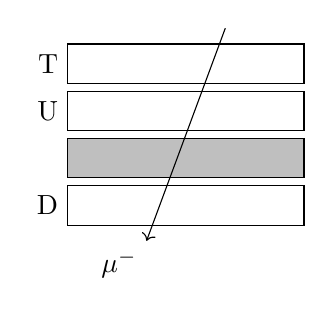
\begin{tikzpicture}
    \draw(0,0)rectangle(3,0.5);
    \fill[lightgray](0,0.6)--(0,1.1)--(3,1.1)--(3,0.6)--cycle;
    \draw(0,0.6)rectangle(3,1.1);
    \draw(0,1.2)rectangle(3,1.7);
    \draw(0,1.8)rectangle(3,2.3);
    \draw[->] (2,2.5)--(1,-0.2) node [below left]{$\mu^{-}$};
    \node [left] at (0,2.05){T};
    \node [left] at (0,1.45){U};
    \node [left] at (0,0.25){D};
\end{tikzpicture}

            \subcaption{試料を通過する場合}
        \end{minipage}
        &
        \begin{minipage}[t]{0.3\hsize}
            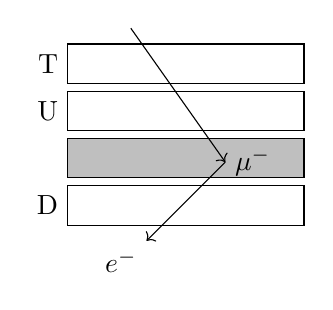
\begin{tikzpicture}
    \draw(0,0)rectangle(3,0.5);
    \fill[lightgray](0,0.6)--(0,1.1)--(3,1.1)--(3,0.6)--cycle;
    \draw(0,0.6)rectangle(3,1.1);
    \draw(0,1.2)rectangle(3,1.7);
    \draw(0,1.8)rectangle(3,2.3);
    \draw[->] (0.8,2.5)--(2,0.8) node [right]{$\mu^{-}$};
    \draw[->] (2,0.8)--(1,-0.2) node [below left]{$e^{-}$};
    \node [left] at (0,2.05){T};
    \node [left] at (0,1.45){U};
    \node [left] at (0,0.25){D};
\end{tikzpicture}

            \subcaption{崩壊してDに(陽)電子を飛ばす場合}
        \end{minipage}
    \end{tabular}
    \caption{PSc+PMTの配置と粒子の飛程}
\end{figure}
\begin{figure}
    \centering
    \begin{circuitikz}
    \draw
    (1,0)
    % BTUnotD
    node[ieeestd and port, number inputs=3, anchor=in 1] (BTUnotD) {}
    % T
    (BTUnotD.in 1) -- ++(-1,0)
    node[anchor=east] {T}
    % GG
    (BTUnotD.out) to[short] ++(0.5,0)
    node[twoportshape, anchor=west, t=GG](GG){} ++(1,0)
    % to D stop
    -- ++(0.5,0)
    to [short, *-] ++(0,-1.5)
    -- ++(1,0)
    node[ieeestd and port, anchor=in 1] (Dstop){}
    (Dstop.out) node[anchor=west]{D stop};
    % not D
    \node at (BTUnotD.bin 3) [ocirc, left]{};
    % GG to U stop
    \draw
    (GG.east)
    to [short] ++(1.5,0)
    node[ieeestd and port, anchor=in 1](Ustop){}
    (Ustop.out) node[anchor=west]{U stop};
    \draw
    (BTUnotD.out) to[short, *-] ++(0,1)
    to[short] ++(5.2,0)
    node[anchor=west](start){start};
    \draw
    (BTUnotD.in 2) to[short] ++(-1,0)
    node[anchor=east](U){U}
    (BTUnotD.in 3) to[short] ++(-1,0)
    node[anchor=east](D){D}
    (0.5,-0.38) to [short, *-] ++(0,-1)
    -- ++(1,0)
    -| (Ustop.in 2)
    (0.7, -0.75) to [short, *-] ++(0,-1.4)
    |- (Dstop.in 2)
    ;
\end{circuitikz}

    \caption{回路の概要}
    \label{img: circuit easy}
\end{figure}
\begin{landscape}
    \begin{figure}
        \centering
        % displaying the circuit without rotation
\begin{circuitikz}
    % B
    \draw
        (1,0)
        % TUnotD
        node[ieeestd and port, number inputs=3, anchor=in 1] (BTUnotD) {}
        % T
        (BTUnotD.in 1) to[short] ++(-1,0)
        node[anchor=east](BT){$\mathrm{CaCO_3}$ T}
        % gateBlocal
        (BTUnotD.out) to[short] ++(0.5,0)
        node[twoportshape, anchor=west, t=GG] (gateBlocal){} ++(1,0)
        % gate delay
        to [short] ++(0.5,0)
        node[align=left, anchor=west](gateBdelay){\small delay\\$\SI{31}{\nano\second}$} ++(1,0)
        % to D stop
        to [short] ++(0.5,0)
        to [short, *-] ++(0,-1.5)
        to [short] ++(0.55,0)
        node[ieeestd and port, anchor=in 1] (BDstoplocal){}
        % (BDstoplocal.out) node[anchor=west]{D stop}
        ;
        % not D
        \node
        at (BTUnotD.bin 3) [ocirc, left]{}
        ;
        % gateBdelay to U stop
        \draw
        (gateBdelay.east)
        to [short] ++(1,0)
        node[ieeestd and port, anchor=in 1](BUstoplocal){} ++(1,0)
        % (BUstoplocal.out) node[anchor=west]{U stop}
        ;
        % start
        \draw
        (BTUnotD.out) to[short, *-] ++(0,1)
        to[short] ++(3.5,0)
        node[anchor=west](Bstart){}
        ;
        \draw
        (BTUnotD.in 2) to[short] ++(-1,0)
        node[anchor=east](U){$\mathrm{CaCO_3}$ U}
        (BTUnotD.in 3) to[short] ++(-1,0)
        node[anchor=east](D){$\mathrm{CaCO_3}$ D}
        (0.5,-0.38) to [short, *-] ++(0,-1)
        -- ++(2,0)
        node[align=left, anchor=west]{\small delay\\ $\SI{2}{\nano\second}$} ++(1,0)
        -| (BUstoplocal.in 2)
        (0.7, -0.75) to [short, *-] ++(0,-1.4)
        |- (BDstoplocal.in 2)
        % node [anchor=north](Ddelay){delay}
        % (Ddelay.east) -- (BDstoplocal.in 2)
        % U stop
        (15,-0.3) node[ieeestd and port, anchor=center, number inputs=3](BUstop){}
        (BUstop.out) node[anchor=west]{$\mathrm{CaCO_3}$ U stop}
        % D stop
        (15,-1.8) node[ieeestd and port, anchor=center, number inputs=3](BDstop){}
        (BDstop.out) node[anchor=west](BDstopLabel){$\mathrm{CaCO_3}$ D stop}
        (BUstoplocal.out) -- (BUstop.in 3)
        (BDstoplocal.out) -- (BDstop.in 3)
        ;
        % box
        \node[rectangle,draw,dashed,fit=(BT) (BDstoplocal) (BDstoplocal)](CaCO3){};
        \node[anchor=north, align=center] at (CaCO3.south){$\mathrm{CaCO_3\:INPUTS}$};
    % A
    \draw
        % T
        (2,6)
        node[ieeestd or port, number inputs=3, anchor=in 1] (ATor) {}
        % T1E
        (0,7) node[anchor=east](T1E){Cu, Al T1}
        -- ++(1.2,0)
        node[align=left, anchor=west](T1Edelay){\small delay\\ $\SI{22}{\nano\second}$} (1,0)
        (T1Edelay.south) |- (ATor.in 1)
        % T2E
        (0,5.62)
        node[anchor=east]{Cu, Al T2}
        -- ++(0.5,0)
        node[align=left, anchor=west](T2Edelay){\small delay\\ $\SI{14}{\nano\second}$} (1,0)
        (T2Edelay.east) -- (ATor.in 2)
        % T3E
        (0,4.5)
        node[anchor=east]{Cu, Al T3}
        -- ++(1.2,0)
        node[align=left, anchor=west](T3Edelay){\small delay\\ $\SI{30}{\nano\second}$}
        (T3Edelay.north) |- (ATor.in 3)
        ;
        \draw
        % TUnotD
        (4.5,3.625)
        node[ieeestd and port, number inputs=3, anchor=in 1](ATUnotD){}
        (ATor.out) |- (ATUnotD.in 1)
        % U
        (ATUnotD.in 2)
        to[short] (0,3.25)
        node[anchor=east]{Cu, Al U}
        % D
        (ATUnotD.in 3)
        to[short] (0,2.9)
        node[anchor=east](AD){Cu, Al D}
        ;
        % not D
        \node at (ATUnotD.bin 3) [ocirc, left]{};
        % AU stop
        \draw
        (15,8) node[ieeestd and port, anchor=center, number inputs=3](AUstop){}
        ;
        \draw
        % U to Ustop
        (3,3.25)
        to [short, *-] ++(0,1.5)
        -| ++(2,3.6)
        -- ++(1,0)
        node[anchor=west, align=left]{\small delay\\ $\SI{30}{\nano\second}$} ++(1,0)
        % to [short] ++(1,0)
        -- (AUstop.in 1)
        % AD stop
        (15,6.5) node[ieeestd and port, anchor=center, number inputs=3](ADstop){}
        ;
        % D to Dstop
        \draw
        (3.5,2.9)
        to [short, *-] ++(0,1.2)
        -| ++(2,3.2)
        to [short] ++(1,0)
        -| (ADstop.in 1)
        (AUstop.out) node[anchor=west](AUstopLabel){Cu, Al U stop}
        (ADstop.out) node[anchor=west]{Cu, Al D stop}
        ;
        % box
        \node[rectangle,draw,dashed,fit=(T1E) (AD) (ATUnotD) (T1Edelay)](CuAl){};
        \node[anchor=north, align=center] at (CuAl.south){Cu, Al INPUTS};
    % gate
    \draw
        % and9
        (10,2.97)
        node[ieeestd and port, anchor=center](and9){}
        % and10
        (10,5)
        node[ieeestd and port, anchor=center](and10){}
        % ATUnotD to 9
        (ATUnotD.out) |- (and9.in 1)
        % gateA
        (8.2,6.5) node[twoportshape, anchor=center, t=GG](gateA){}
        % gateB
        (8.2,1) node[twoportshape, anchor=center, t=GG](gateB){}
        (Bstart.west) |- (and10.in 2)
        % start trigger
        (15,4)
        node[ieeestd or port, anchor=center](STARTor){}
        (STARTor.out) node[anchor=west]{start}
        % 9 and 10 to start or
        (and9.out) |- (STARTor.in 2)
        (and10.out) |- (STARTor.in 1)
        % 9 to gate A
        (and9.out) to [short, *-] ++(0,-1)
        to [short] ++(-4,0)
        |- (gateA.west)
        % 10 to gate B
        (and10.out) to [short, *-] ++(0,0.9)
        to [short] ++(-3.7,0)
        |- (gateB.west)
        ;
        \draw
        % gate B to BU stop
        (gateB.east) to[short, -*] (13,1)
        |- (BDstop.in 2)
        % gate B to BD stop
        (13,-0.3) to[short, *-] (BUstop.in 2)
        % gate B to A stop
        (gateB.east) -- (13,1)
        |- (AUstop.in 3)
        (13,6.13) to[short, *-] (ADstop.in 3)
        ;
        \node
        at (AUstop.bin 3) [ocirc, left]{}
        ;
        \node
        at (ADstop.bin 3) [ocirc, left]{}
        ;
        % gate B to 9
        \draw
        (gateB.east) to[short] ++(0.2,0)
        to [short, *-] ++(0,0.2)
        |- (and9.in 2)
        ;
        \node
        at (and9.bin 2) [ocirc, left]{}
        ;
        % gate A to 10
        \draw
        (gateA.east) to[short] ++(0.2,0)
        to [short, *-] ++(0,-0.2)
        |- (and10.in 1)
        ;
        \node
        at (and10.bin 1) [ocirc, left]{}
        ;
        \draw
        % gate A to A stop
        (12,6.5) to[short, *-] ++(0,1.5)
        -- (AUstop.in 2)
        (12,6.5) -- (ADstop.in 2)
        % gate A to B stop
        (gateA.east) to[short] (12,6.5)
        |- (BDstop.in 1)
        ;
        \node
        at (BDstop.bin 1) [ocirc, left]{}
        ;
        \draw
        (12,0.06) to[short, *-] (BUstop.in 1)
        ;
        \node
        at (BUstop.bin 1) [ocirc, left]{}
        ;
        % box
        \node[rectangle,draw,dashed,fit=(gateA) (gateB) (and9) (and10)](gates){};
        \node[anchor=north east, align=left] at (gates.south east){GATES};
    % outputs box
    \node[rectangle,draw,dashed,fit=(AUstop)(BDstop)(AUstopLabel)(BDstopLabel)](outputs){};
    \node[anchor=north, align=center]at(outputs.south){OUTPUTS};
\end{circuitikz}

        \caption{実験で用いた論理回路}
    \end{figure}
\end{landscape}
\end{document}
